\documentclass{classrep}
\usepackage[utf8]{inputenc}
\frenchspacing

\usepackage{graphicx}
\usepackage[usenames,dvipsnames]{color}
\usepackage[hidelinks]{hyperref}
\usepackage{float}

\usepackage{amsmath, amssymb, mathtools}

\usepackage{fancyhdr, lastpage}
\pagestyle{fancyplain}
\fancyhf{}
\renewcommand{\headrulewidth}{0pt}
\cfoot{\thepage\ / \pageref*{LastPage}}


\studycycle{Informatyka stosowana, studia dzienne, II st.}
\coursesemester{I}

\coursename{Języki programowania w Analizie Danych}
\courseyear{2019/2020}

\courseteacher{dr inż. Krzysztof Lichy}
\coursegroup{poniedziałek, 14:15}

\author{%
  \studentinfo[234102@edu.p.lodz.pl]{Zbigniew Nowacki}{234102}\\
  \studentinfo[234067@edu.p.lodz.pl]{Bartosz Jurczewski}{234067}%
}

\title{Zadanie 1: Analiza statystyczna}

\begin{document}
\maketitle
\thispagestyle{fancyplain}
\section{Cel}
Celem zadania było przeprowadzenie analizy statystycznej dla wybranych zbiorach danych.

\section{Wprowadzenie}
Plik \textit{main3.py} zawiera skrypt realizujący następujące wymagania:
\begin{enumerate}
    \item Dla poszczególnych atrybutów wyznaczyć medianę, minimum i maximum dla cech ilościowych oraz dominantę dla cech jakościowych.
    \item Narysować histogramy dla dwóch cech ilościowych najbardziej ze sobą skorelowanych.
    \item Zadbać o czytelność rezultatów oraz staranny i atrakcyjny wygląd histogramów.
\end{enumerate}
\vspace{0.5cm}
\par Plik \textit{main4.py} zawiera skrypt realizujący następujące wymagania:
\begin{enumerate}
    \item Zbadać jedną z następujących hipotez:
    \begin{enumerate}
        \item Dla danych Births zbadać hipotezę, że dzienna średnia liczba urodzeń dzieci wynosi: 10000.
        \item Dla danych manaus zbadać hipotezę, że średnia wysokość rzeki w manaus jest na wysokości punktu arbitralnego(wynosi 0).
        \item Dla danych quakes zbadać hipotezę, że średnia głębokość występowania trzęsienia ziemi wynosi 300 metrów. 
    \end{enumerate}
    \item Zwizualizować rozkłady na histogramie.
    \item Zaznaczyć na wykresie punkt dotyczący badanej hipotezy.
\end{enumerate}

\section{Opis implementacji}
Zadanie zostało zrealizowane przy użyciu języka \textbf{Python} w wersji 3.7, z wykorzystaniem bibliotek: \textit{pandas}, \textit{matplotlib} i \textit{scipy}.

\section{Wyniki}
\subsection{Cześć 1 - ocena dostateczna}

Do spełnienia wymagań na ocenę dostateczną wybraliśmy zbiór \textit{iris.data}.
\textit{Sepal length} to długość działki kielicha, a \textit{petal width} to szerokość płatku irisa.

Wyniki dla poszczególnych atrybutów (cech ilościowych):

%%% Mediana
\begin{table}[H]
    \centering
    \begin{tabular}{|c|c|}
    \hline
    \multicolumn{2}{|c|}{\textbf{Mediana}} \\ \hline
    sepal length           & 5.80          \\ \hline
    sepal width            & 3.00          \\ \hline
    petal length           & 4.35          \\ \hline
    petal width            & 1.30          \\ \hline
    \end{tabular}
    \caption{Mediany dla poszczególnych atrybutów ze zbioru \textit{iris.data}}
    \label{tab:w1}
\end{table}

%%% Minimum
\begin{table}[H]
    \centering
    \begin{tabular}{|c|c|}
    \hline
    \multicolumn{2}{|c|}{\textbf{Minimum}} \\ \hline
    sepal length           & 4.3           \\ \hline
    sepal width            & 2.0           \\ \hline
    petal length           & 1.0           \\ \hline
    petal width            & 0.1           \\ \hline
    \end{tabular}
    \caption{Minima dla poszczególnych atrybutów ze zbioru \textit{iris.data}}
    \label{tab:w2}
\end{table}

%%% Maksimum
\begin{table}[H]
    \centering 
    \begin{tabular}{|c|c|}
    \hline
    \multicolumn{2}{|c|}{\textbf{Maksimum}} \\ \hline
    sepal length           & 7.9           \\ \hline
    sepal width            & 4.4           \\ \hline
    petal length           & 6.9           \\ \hline
    petal width            & 2.5           \\ \hline
    \end{tabular}
    \caption{Maksima dla poszczególnych atrybutów ze zbioru }
    \label{tab:w3}
\end{table}

Dominantą dla cechy jakościowej czyli gatunkiem są \textit{Iris-setosa}, \textit{Iris-versicolor} i \textit{Iris-virginica}. Wynika to z specyfiki danych - w pliku znajduję się po 50 irysów z każdego gatunku.

\vspace{1cm}

Dwie cechy ilościowe najbardziej skorelowane ze sobą to \textit{petal length} i \textit{petal width}. Ich relacja została pokazana na rysunku \ref{fig:hist3}.

\begin{figure}[H]
    	\centering
    	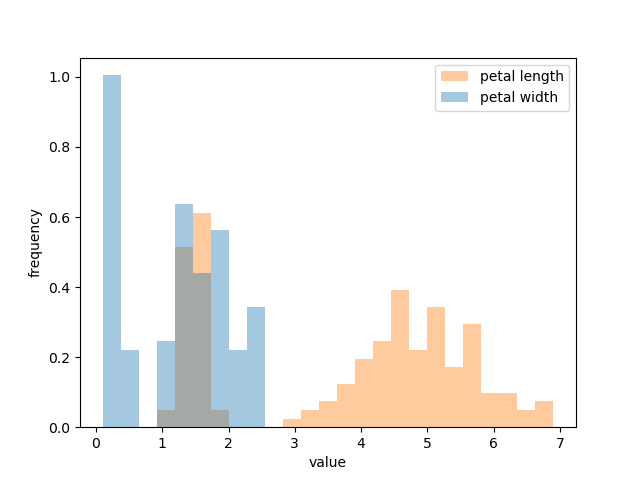
\includegraphics[width=0.8\textwidth]{images/histogram3.png}
    	\caption{Histogram dla danych \textit{iris}}
    	\label{fig:hist3}
\end{figure}

\subsection{Cześć 2 - ocena dobra} \label{sec:badania2}

Zbiór danych: \textit{quakes}.\\
Hipoteza: "średnia głębokość występowania trzęsienia ziemi wynosi 300 metrów".
\begin{figure}[H]
    	\centering
    	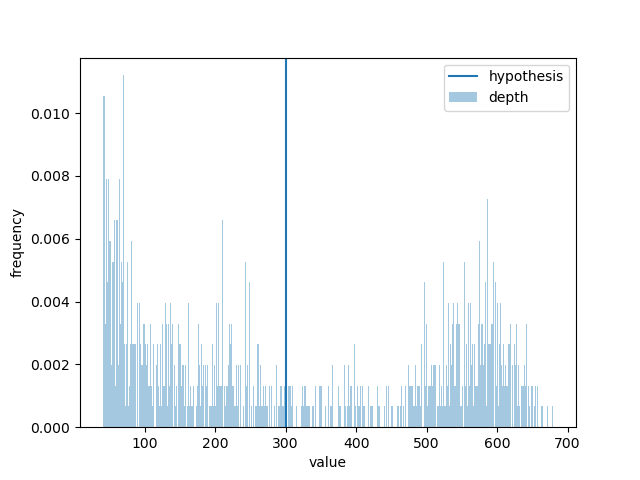
\includegraphics[width=0.8\textwidth]{images/histogram4.png}
    	\caption{Histogram dla danych \textit{quakes}}
    	\label{fig:hist4}
\end{figure}

% \begin{table}[H]
%     \centering
%     \begin{tabular}{|l|l|}
%     \hline
%     \textbf{T-Statistic:} & 5674.57 \\ \hline
%     \textbf{P-Value:}     & 0.0               \\ \hline
%     \end{tabular}
%     \caption{}
%     \label{tab:1}
% \end{table}

Próbka danych na której badano hipotezę nie pochodzi z rozkładu normalnego. Wnioski wyciągnięte na podstawie takiej próbki należy odrzucić.

% \section{Dyskusja}
% Przeprowadzone przez nas badania

\section{Wnioski}
\begin{itemize}
    \item Korzystanie z gotowych bibliotek do statystki znacznie przyspieszyło i ułatwiło pracę z danymi.
    \item Program oblicza poprawnie podstawowe funkcje statystyczne.
    \item Przed rozpoczęciem opracowania wyników należy upewnić się że próbka pochodzi z rozkładu normalnego.
\end{itemize}

\begin{thebibliography}{0}
    \bibitem{dagostino}
    \textsl{An Omnibus Test of Normality for Moderate and Large Size Samples}, 1971, Ralph B. D'Agostino, \url{https://pdfs.semanticscholar.org/1493/2aec5e2128d2373d57f6dede6c3c7ed71f07.pdf}
    \bibitem{fuw}
    \textsl{WnioskowanieStatystyczne/ Testowanie hipotez, \url{https://brain.fuw.edu.pl/edu/index.php/WnioskowanieStatystyczne/_Testowanie_hipotez\#Przyk.C5.82ad_.28zastosowanie_r.C3.B3.C5.BCnych_test.C3.B3w_do_tych_samych_danych.29:_karma}}
    \bibitem{wosiak}
    \textsl{A. Wosiak – Języki programowania w analizie danych, \url{https://ftims.edu.p.lodz.pl/pluginfile.php/136679/mod_resource/content/1/Python_wyklad_02_Statystyka.pdf}}
    \bibitem{ttest}
    \textsl{\url{https://www.statisticshowto.datasciencecentral.com/probability-and-statistics/t-test/}}
\end{thebibliography}

\end{document}
